\section{Method}\label{sec:method}

The computational workflows were run at scale using the REANA reusable analysis platform~\cite{ref:chep2018}.
The computational backend was the Kubernetes cluster of various sizes (from 500 cores up to 5000 cores).
We have been varying several parameters of the cluster such as the number of nodes and the required memory and studied the maximum number of pMSSM workflows that the platform can handle concurrently.
After performing several such computational experiments, we have improved the scheduling efficiency of REANA to increase the running bandwidth for the pMSSM style of workflows.

\begin{figure}
\centering
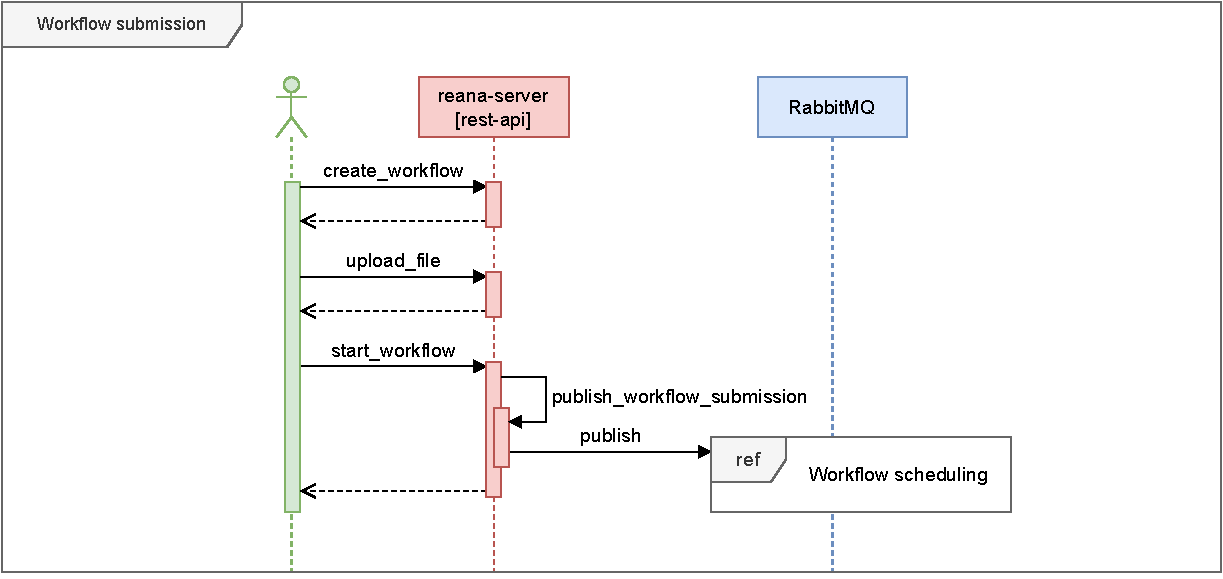
\includegraphics[width=0.9\textwidth]{sequence-submission.pdf}
\caption{The sequence diagram showing how REANA schedules incoming workflows after submission.
The submitted workflows are announced via message queue that is later processed by the workflow scheduler in Figure~\ref{fig:reanascheduler2}.}
\label{fig:reanascheduler1}
\end{figure}

Figure~\ref{fig:reanascheduler1} shows the sequence diagram of the workflow submission stage.
The incoming workflows are stored in a queue that is later processed by the scheduler.
The first task was to improve the performance of the REANA platform's server submission end points to allow many concurrent workflow starting requests.

\begin{figure}
\centering
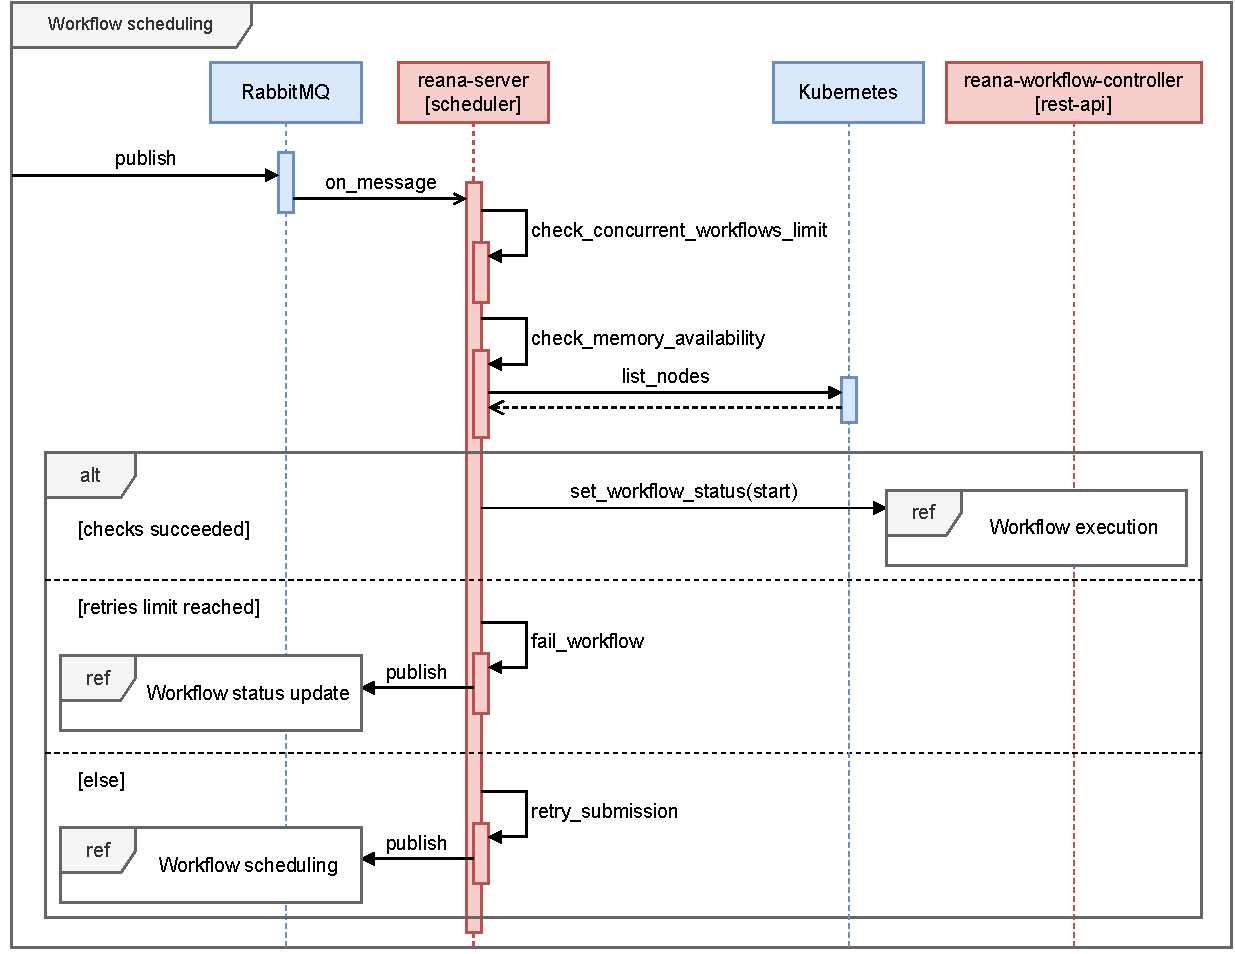
\includegraphics[width=0.9\textwidth]{sequence-scheduling.pdf}
\caption{The sequence diagram showing how REANA schedules queued workflows.
The system checks for available resources before allowing workflow runs for execution.
The checking and rescheduling workflow offers several possibilities for optimisations.
The workflows accepted for execution are further processed in Figure~\ref{fig:reanascheduler3}.}
\label{fig:reanascheduler2}
\end{figure}

Figure~\ref{fig:reanascheduler2} shows the next stage of the process, namely how the submitted workflows are being consumed from the incoming queue.
The scheduler first checks whether the incoming workflow does not exceed the limits on the total number of workflow the system could handle as well as currently available free memory on the Kubernetes cluster.
If the checks succeed, the workflow is accepted for execution.
In the opposite case the incoming workflow is being rescheduled and attempted to be accepted for execution several times whilst waiting for the Kubernetes cluster resources to liberate.
If the workflow cannot be scheduled for a substantial amount of time, a failure is declared.

\begin{figure}
\centering
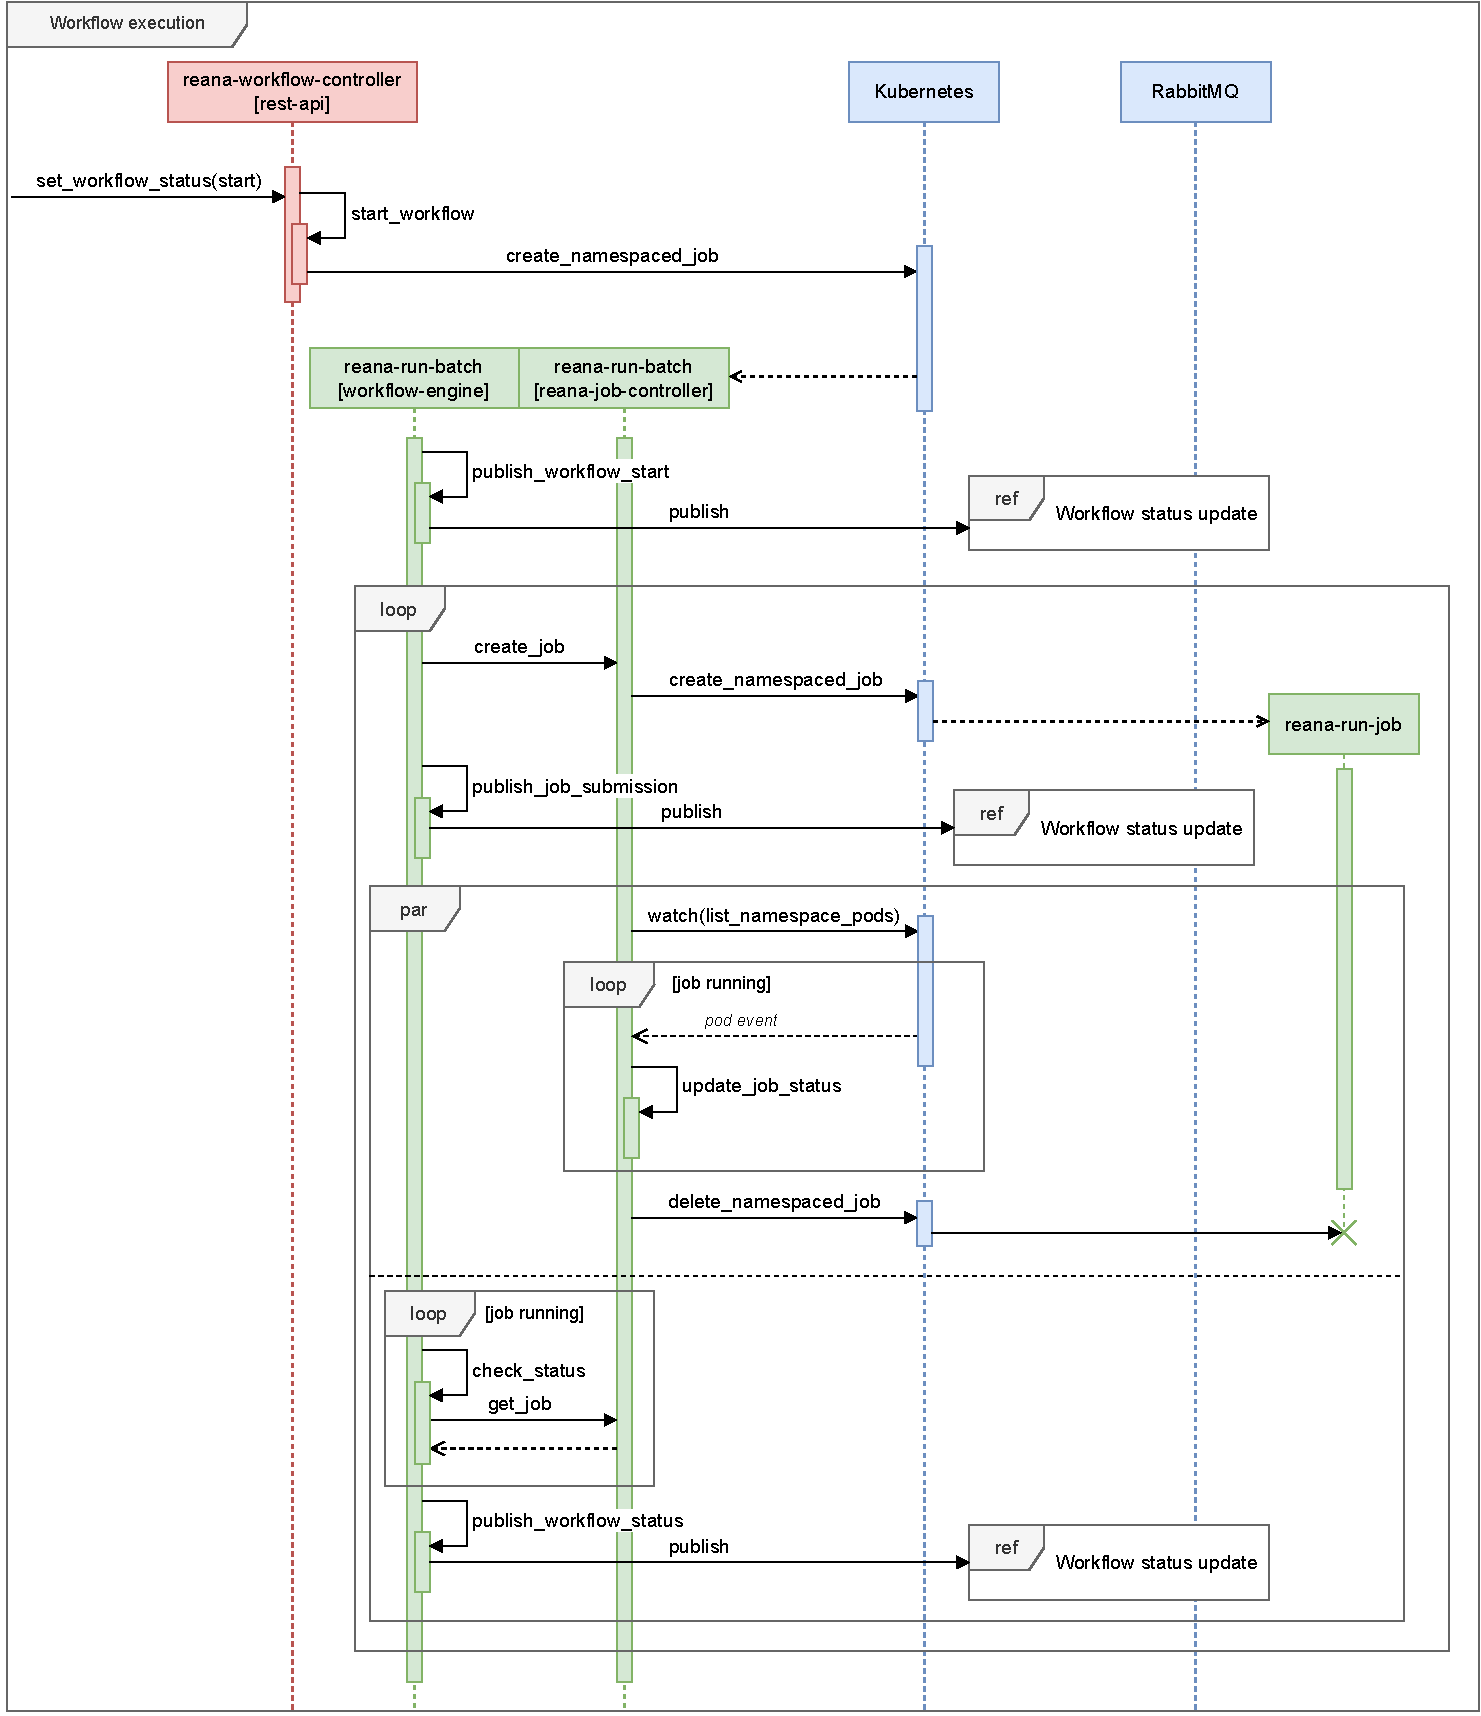
\includegraphics[width=0.95\textwidth]{sequence-execution.pdf}
\caption{The sequence diagram showing how the REANA executes scheduled workflows.
Note the interplay between the scheduler and the Kubernetes cluster.
The pod creation offers another space for optimisations.
The workflow execution status monitoring is carried out by a watching loop.
The workflow jobs are started for each workflow step.
The termination procedures are further illustrated in Figure~\ref{fig:reanascheduler4}.}
\label{fig:reanascheduler3}
\end{figure}

Figure~\ref{fig:reanascheduler3} shows the stage of the running of the workflow after it has been accepted for execution.
Note the interplay of the REANA platform with the underlying Kubernetes cluster: the job is scheduled using the Kubernetes native job scheduler mechanism which include additional scheduling delays that needed to be taken into account for optimisation.
The progress of the workflow is monitored until the workflow execution terminates.
The workflow steps are launched when the worker nodes are free to run the workload.
The status of jobs is published in the message queue.

\begin{figure}
\centering
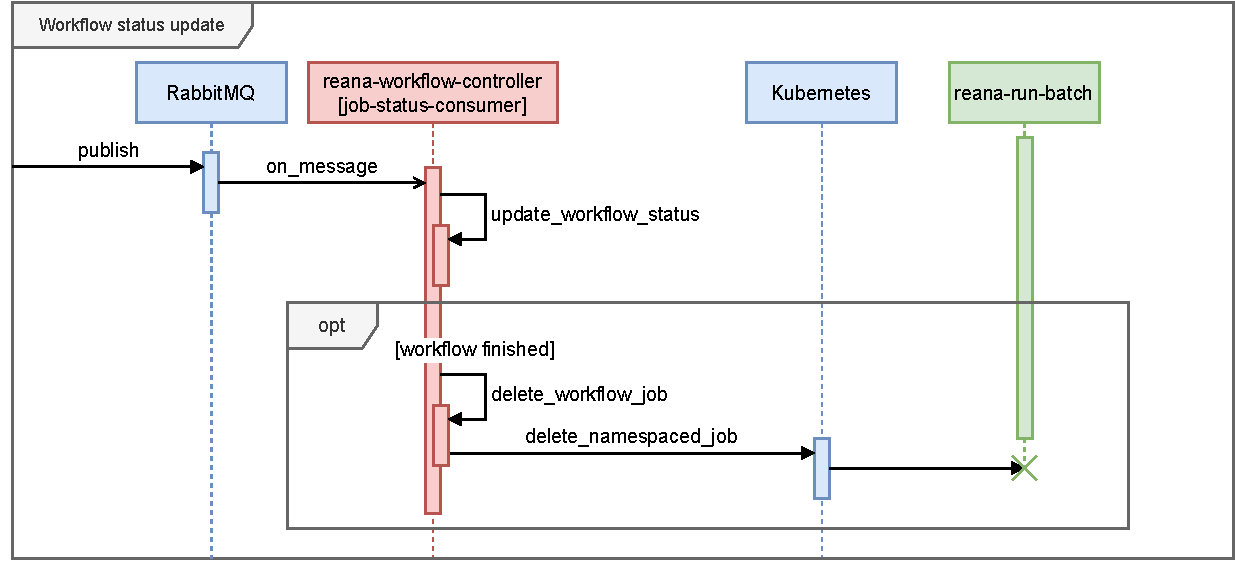
\includegraphics[width=0.9\textwidth]{sequence-termination.pdf}
\caption{The sequence diagram showing how REANA updates workflow statuses and terminates finished workflows.
The procedure involves consuming the message queue, closing the Kubernetes pods, and updating the database about the status of the workflow run.
In case of launching several thousands of concurrent workflows, these processes also have to be optimised.}
\label{fig:reanascheduler4}
\end{figure}

Figure~\ref{fig:reanascheduler4} shows the termination stage of the workflow.
When all the steps are finished and the results are produced, the system has to delete the Kubernetes pod and update the status of the workflow in both the message queue and the database.
This constituted another layer of optimisations in order to handle any status handling processes in an asynchronous manner whilst the platform is starting the new incoming workflows.
